\begin{figure}[!htbp]
    \centering
    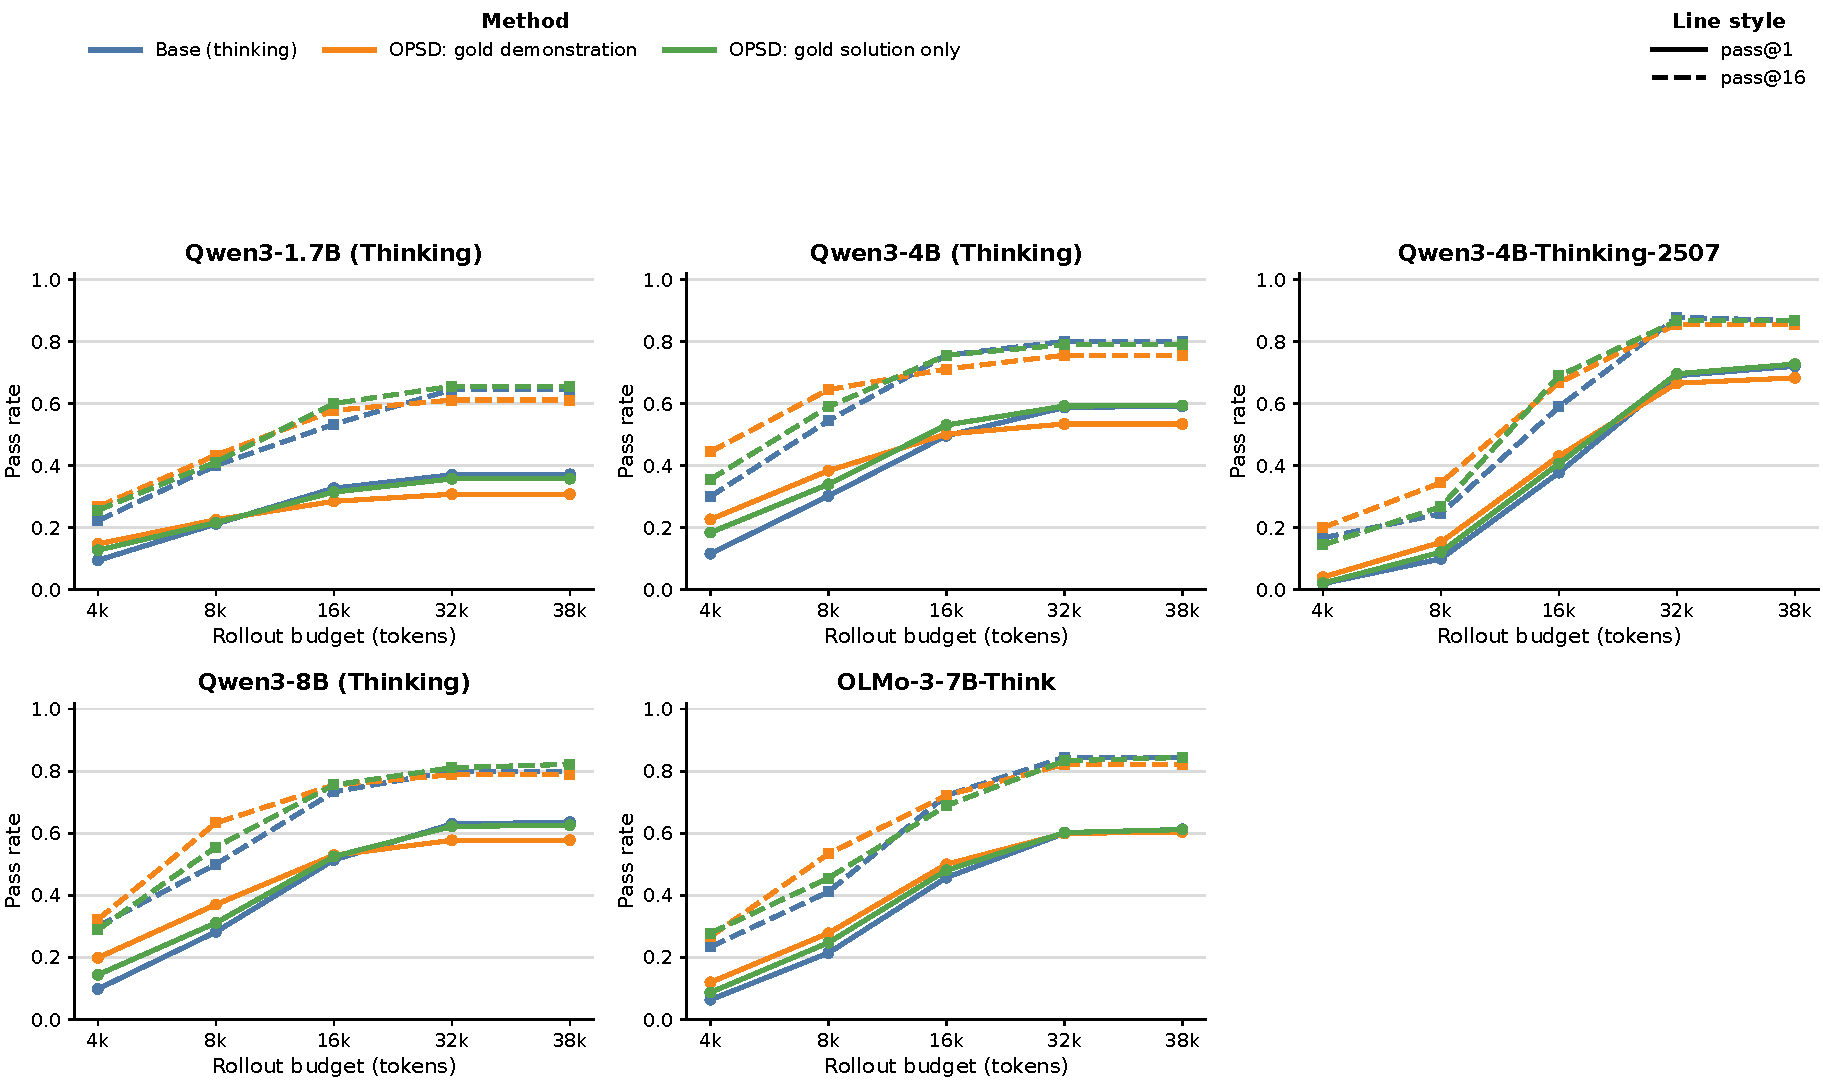
\includegraphics[width=\linewidth]{figures/avg_pass_budget_curves_thinking5_fs_ao.pdf}
    \caption{
    \textbf{Per-model pass-rate budget curves separate the accuracy effects in Figure~\ref{fig:openthoughts_accuracy_length_collapse}.}
    We evaluate five OpenThoughts-trained thinking models at rollout budgets from 4k to 38k tokens on AIME24, AIME25, and HMMT25.
    Solid lines show pass@1 and dashed lines show pass@16.
    Blue curves are base thinking models, orange curves are \opsd{} with full gold-demonstration context, and green curves are \opsd{} with final-answer-only privileged context.
    Dense demonstrations tend to give larger short-budget gains, while the advantage narrows or reverses at longer budgets for several models.
    }
    \label{fig:openthoughts_budget_pass_rates_thinking5_fs_ao}
\end{figure}
